\section{\emph{Hello World}: writing your first JSBML applications}

This section presents two examples for using JSBML. One example reads an
existing \texttt{SBMLDocument} from a file an visualizes it on a \texttt{JFrame}.
The second example creates a new \texttt{SBMLDocument} from scratch and writes
its content into a file. This should help you getting started and writing your
own JSBML applications.

\subsection{Reading and visualizing an \texttt{SBMLDocument}}

Listing~\vref{lst:Visualization} demonstrates in a simple code example how to
parse an SBML file\index{SBML!XML file} (submitted as first argument) and to
immediately display its content on a \texttt{JFrame}.
\index{graphical user interface!\texttt{JFrame}}%
\lstinputlisting[language=Java,float,caption={Parsing and visualizing the
content of an SBML file},
label=lst:Visualization]{%
../publications/Bioinformatics2011ApplicationNote/src/JSBMLvisualizer.java}
\begin{SCfigure}[][h]
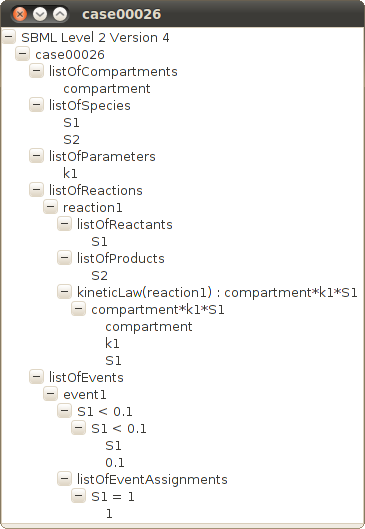
\includegraphics[width=.35\textwidth]{%
../posters/2010_ICSB_and_COMBINE/JSBMLvisualizerTransparent.png}
\caption[Tree representation of an SBML file]{A tree representation of the
content of SBML test model \texttt{case00026}. In JSBML, the hierarchically
structured \texttt{SBMLDocument} can be traversed recursively because all
instances of \texttt{SBase} implement the interface \texttt{TreeNode}.}
\label{fig:Visualization}
\end{SCfigure}
Fig.~\vref{fig:Visualization} shows an example output when applying the program
to an SBML test model.
\index{SBML!test cases}%
Line 16 in Listing~\vref{lst:Visualization} shows how to read an
\texttt{SBMLDocument} from a file, using the \texttt{SBMLReader}. Afterwards,
the \texttt{JSBMLvisualizer} constructor is called, which first creates a new
\texttt{JFrame} with the model's id as title (line 9). Since JSBML's
\texttt{SBase} object, and all derived elements, implement the \texttt{TreeNode}
interface, it is possible to create a \texttt{JTree} from the information in the
\texttt{SBMLDocument} only. This is done in line 10.

\subsection{Creating and writing an \texttt{SBMLDocument}}

\lstinputlisting[language=Java,float,caption={Creating a new
\texttt{SBMLDocument} and writing its content into a file},
label=lst:Creation]{src/JSBMLexample.java}
Listing~\vref{lst:Creation} shows a more complex example. A new
\texttt{SBMLDocument} is created from scratch. It mainly consists of one
\texttt{Compartment}, one \texttt{Model}, two \texttt{Species}, and a
\texttt{Reaction} in which both \texttt{Species} are involved. This
\texttt{SBMLDocument} is written into a file, using \texttt{SBMLWriter}.


\subsection{Further examples}

Listing~\vref{lst:LibSBMLio} shows how to convert libSBML data structures into
JSBML data objects. Listing~\vref{lst:PluginAction} demonstrates the
implementation of CellDesigner's abstract class \texttt{PluginAction} and
Listing~\vref{lst:Plugin} gives a complete example for writing CellDesigner
plugins with JSBML.
